% flashcards-title: One group of ten counters and two single counters
% flashcards-desc: Ten counters are enclosed in one rounded rectangle. Two more counters sit separately to its right.
\documentclass[dvisvgm,tikz,border=8pt]{standalone}
\usetikzlibrary{arrows.meta,patterns}

\definecolor{qraNavy}{HTML}{17324D}
\definecolor{qraBlue}{HTML}{2B6CB0}
\definecolor{qraGold}{HTML}{B7791F}
\definecolor{qraPale}{HTML}{EAF2F8}
\definecolor{qraGray}{HTML}{5C6773}

\tikzset{
  qra axis/.style={draw=qraNavy, line width=1.2pt},
  qra tick/.style={draw=qraNavy, line width=1pt},
  qra guide/.style={draw=qraGray, densely dashed, line width=0.8pt},
  qra counter/.style={circle, draw=qraNavy, fill=qraPale, line width=0.9pt, minimum size=7mm, inner sep=0pt},
  qra label/.style={font=\sffamily\bfseries, text=qraNavy},
  qra small label/.style={font=\sffamily, text=qraNavy},
}

\begin{document}
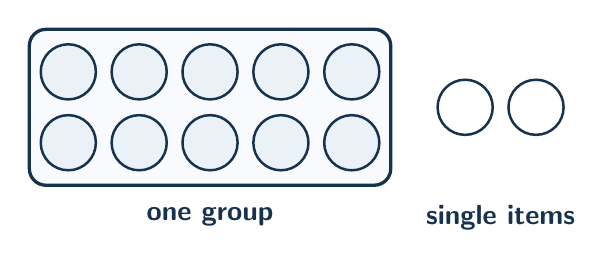
\begin{tikzpicture}[x=0.9cm,y=0.9cm]
  \draw[qra axis, rounded corners=6pt, fill=qraPale!35] (-0.55,-0.6) rectangle (4.55,1.6);
  \foreach \x in {0,1,2,3,4} {
    \node[qra counter] at (\x,1) {};
    \node[qra counter] at (\x,0) {};
  }
  \node[qra counter, fill=white] at (5.6,0.5) {};
  \node[qra counter, fill=white] at (6.6,0.5) {};
  \node[qra label] at (2,-1.05) {one group};
  \node[qra label] at (6.1,-1.05) {single items};
\end{tikzpicture}
\end{document}
